%!TEX root = ./slides-09-rd.tex
%%%%%%%%%%%%%%%%%%%%%%%%%%%%%%%%%%%%%%%%%%%%%%%%%%%%%%%%%%%%%%%%%%%%%%%%%%%%%%%%
\begin{frame}{Centering running variable}

Common for authors to ``re-center'' running variable $X_i$ by subtracting the cut-off, $c_0$. 

\begin{align*}
    Y_i &= \beta_0 + \beta_1 X_i + \delta D_i + \epsilon_i \\
    \implies Y_i &= \beta_0 + \beta_1 (X_i - c_0) + \delta D_i + \epsilon_i \\
    =& (\beta_0 - \beta_1 \cdot c_0) + \beta_1 X_i + \delta D_i + \epsilon_i \\
    =& \alpha + \beta_1 X_i + \delta D_i + \epsilon_i
\end{align*}
Variables can maintain the same interpretation if we re-center the running variable $X_i$ and change the intercept


\end{frame}

%%%%%%%%%%%%%%%%%%%%%%%%%%%%%%%%%%%%%%%%%%%%%%%%%%%%%%%%%%%%%%%%%%%%%%%%%%%%%%%%
\begin{frame}{Linear Sharp RDD}

\textbf{Goal: } estimate treatment effect at the cut-off, $c_0$


\begin{itemize}
    \item Many sharp RDDs are nonlinear, but it's helpful to start thinking about estimation in a linear model:
\end{itemize}
\begin{equation*}
    Y_i = \beta_0 + \beta_1 X_i + \beta_2 \mathbf{1}\{X_i > c_0\} +  \beta_3  \mathbf{1}\{X_i > c_0\} X_i
\end{equation*}
\begin{itemize}
    \item Estimating this equation is the same as estimating a linear model above and below the threshold
    \begin{itemize}
        \item $\beta_0$ is intercept before cut-off
        \item $\beta_0 + \beta_2$ is intercept after cut-off
    \end{itemize}
\end{itemize}
Why do we re-center the running variable $X_i$?
\begin{itemize}
    \item If you re-center the model, $\beta_0$ is the predicted value at the threshold, for the values below $c_0$
    \begin{equation*}
        \beta_0 = \lim_{x \uparrow c} \EE [Y \vert X_i = x]
    \end{equation*}
    \item Then $\beta_0 + \beta_2$ is the predicted value at the threshold, for values above $c_0$
    \begin{equation*}
        \beta_0 + \beta_2 = \lim_{x \downarrow c} \EE [Y \vert X_i = x]
    \end{equation*}
\end{itemize}
$\implies$ ATE equals $\beta_2$

\end{frame}



%%%%%%%%%%%%%%%%%%%%%%%%%%%%%%%%%%%%%%%%%%%%%%%%%%%%%%%%%%%%%%%%%%%%%%%%%%%%%%%%
\begin{frame}{Nonlinearities}

\begin{columns}
\begin{column}{.5\textwidth}
\begin{figure}
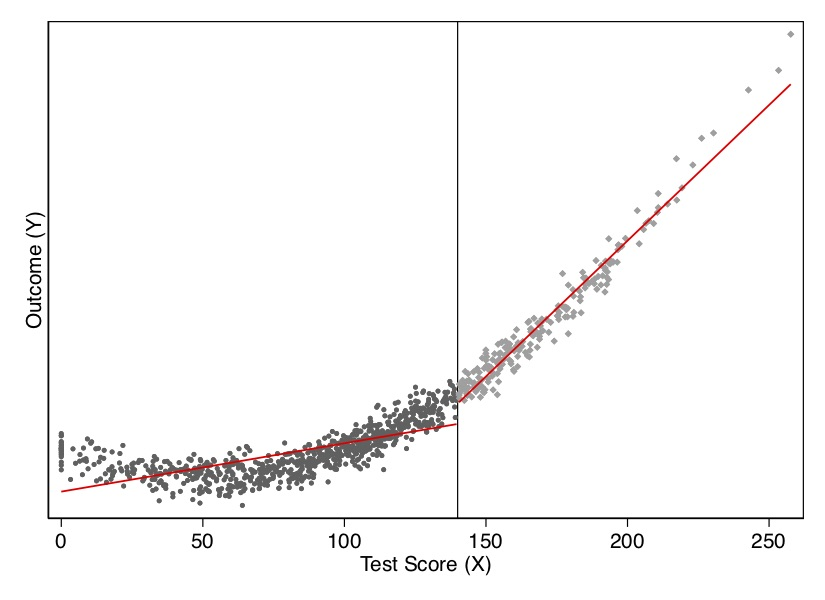
\includegraphics[scale=0.2]{img/rdd_simul4.jpg}
\end{figure}
\end{column}
\begin{column}{.5\textwidth}
\begin{itemize}
    \item True data generating process is nonlinear
    \item Using a linear model may lead to a spurious example
    \item On the left: fitting a model using a least squares regression controlling for the running variable estimates a causal effect though there isn’t one
\end{itemize}
\end{column}
\end{columns}

\end{frame}

%%%%%%%%%%%%%%%%%%%%%%%%%%%%%%%%%%%%%%%%%%%%%%%%%%%%%%%%%%%%%%%%%%%%%%%%%%%%%%%%
\begin{frame}{Nonlinearities}

Suppose the nonlinear relationship is:
\begin{equation*}
    \EE [Y_i (0) \vert X_i] = f(X_i),
\end{equation*}
where $f (X_i)$ is a reasonably smooth function of $X_i$. Then fit the regression model:
\begin{equation*}
    Y_i = f(X_i) + \delta D_i + \epsilon_i
\end{equation*}
Question: since $f(X_i)$ is unobservable for $X_i > c_0$, how do you model the nonlinearity?
\begin{enumerate}
    \item Estimate $f(X_i)$ using a $p$-th order polynomial
    \item Nonparametric kernel estimation
\end{enumerate}


\end{frame}

%%%%%%%%%%%%%%%%%%%%%%%%%%%%%%%%%%%%%%%%%%%%%%%%%%%%%%%%%%%%%%%%%%%%%%%%%%%%%%%%
\begin{frame}{Nonlinear estimation: polynomial}

Generate $f(X_i)$ by allowing $X_i$ to differ on both sides of the cutoff. Letting $\tilde{X}_i$ be the centered running variable:
\begin{align*}
    \EE [Y_i (0) \vert X_i] &= \alpha + \beta_{01} \tilde{X}_i + \beta_{02} \tilde{X}_i^2 + \dots + \beta_{0p} \tilde{X}_i^p \\
    \EE [Y_i (1) \vert X_i] &= \alpha + \delta + \beta_{11} \tilde{X}_i + \beta_{12} \tilde{X}_i^2 + \dots + \beta_{1p} \tilde{X}_i^p \\
\end{align*}
Translating this into observed $Y_i$:
\begin{align*}
    \EE [Y_i \vert X_i] &= 
    \EE [Y_i (0) \vert X_i] + \Big( \EE [Y_i (1) \vert X_i] - \EE [Y_i (0) \vert X_i] \Big) D_i 
\end{align*}
Regression model given by:
\begin{equation*}
    Y_i = \alpha + \beta_{01} \tilde{X}_i + \beta_{02} \tilde{X}_i^2 + \dots + \beta_{0p} \tilde{X}_i^p
    + \delta D_i
    + \beta_{1}^* D_i \tilde{X}_i + \beta_{2}^* D_i \tilde{X}_i^2 + \dots + \beta_{p}^* D_i \tilde{X}_i^p + \epsilon_i
\end{equation*}
where $\beta_{p}^* = \beta_{1p} - \beta_{0p}$. 
\begin{itemize}
    \item At $c_0$, treatment effect given by $\delta$
    \item At $c > c_0$, treatment effect given by $\delta + \beta_1^* c + \beta_2^* c^2 + \dots + \beta_p^* c^p$
    % \item At $X_i > c_0$, treatment effect given by $\delta + \beta_1^* c$
\end{itemize}

\end{frame}

%%%%%%%%%%%%%%%%%%%%%%%%%%%%%%%%%%%%%%%%%%%%%%%%%%%%%%%%%%%%%%%%%%%%%%%%%%%%%%%%
\begin{frame}{Nonlinear estimation: polynomial}


Validity of RDD estimates using polynomials depends on whether polynomial model provides an accurdate description of $\EE[Y_i (0) \vert X_i]$
\begin{itemize}
    \item If polynomial model is not appropriate, then what looks like a jump might actually just be unaccounted for nonlinearity
\end{itemize}

\vspace{3ex}
\href{https://doi.org/10.1080/07350015.2017.1366909}{Gelman and Imbens (2019)}: ``Why High-Order Polynomials Should Not Be Used in Regression Discontinuity Designs''
\begin{itemize}
    \item Controlling for higher-order polynomials (3+) can lead to nonsensical results
    \item Three major problems: 
    \begin{itemize}
        \item Noisy estimates
        \item Sensitivity to degree of the polynomial
        \item Poor coverage of confidence intervals
    \end{itemize}
    \item Authors recommend local linear or quadratic polynomials or other smooth functions
\end{itemize}

\vspace{3ex}
That said, it's conceptually important, and used in older papers!
% so we'll review it: \textbf{Example notebook}

\end{frame}

%%%%%%%%%%%%%%%%%%%%%%%%%%%%%%%%%%%%%%%%%%%%%%%%%%%%%%%%%%%%%%%%%%%%%%%%%%%%%%%%
\begin{frame}{Nonlinear estimation: kernel estimation}

Kernel regression provides an alternative to using higher-order polynomials

\vspace{3ex}
Regression Discontinuity relies heavily on the extrapolation 
\begin{itemize}
    \item Looking at the values at the beginning and end of 2 regression lines
    \item If regression is focusing on fitting other data points, rather than correctly fitting at the threshold, the treatment effect might be misspecified
\end{itemize}

\vspace{3ex}
\textbf{Possible solution:} give higher weights to points close to the cutoff $c_0$

\vspace{3ex}
\href{https://doi.org/10.1111/1468-0262.00183}{Hahn, Todd, and Van der Klaauw (2001)}: 
\begin{itemize}
    \item To avoid poor boundary performance, use weighted regression restricted to a window (``local'') 
    % \item Local linear estimators have better boundary properties than the traditional kernel regression estimat 
    \item In local kernel regression: ``kernel'' provides weights close to the cut-off; can then use weighted least squares to estimate effects
\end{itemize}


\end{frame}



%%%%%%%%%%%%%%%%%%%%%%%%%%%%%%%%%%%%%%%%%%%%%%%%%%%%%%%%%%%%%%%%%%%%%%%%%%%%%%%%
\begin{frame}{Kernel weighting function}

Re-weight sample using the \textbf{triangle kernel}:
\begin{equation*}
    K (X, c_0, h) = \mathbf{1} \{ \vert X - c_0 \vert \leq h\} \cdot \left( 1 - \frac{X - c_0}{h} \right)
\end{equation*}
\begin{itemize}
    \item $\vert X - c_0 \vert \leq h$: The absolute difference between $X$ and $c_0$ is less than or equal to some \textbf{bandwidth} $h$
    \item $\mathbf{1} \{ \vert X - c_0 \vert \leq h\}$: Indicator function that equals 1 if X is sufficiently close to $c_0$, according to the bandwidth $h$; 0 otherwise
    \item $\left( 1 - \frac{X - c_0}{h} \right)$: re-weighting function
    \begin{itemize}
        \item Ignore cases where $X - c_0 > h$, because of the indicator function
        \item We know $(X - c_0) / h$ is less than or equal to 1
        \item The further $X$ is from $c$, the larger this fraction is
        \item Because this fraction is subtracted from 1, the weights get smaller the farter $X$ is from the cut-off
    \end{itemize}
\end{itemize}



\end{frame}


%%%%%%%%%%%%%%%%%%%%%%%%%%%%%%%%%%%%%%%%%%%%%%%%%%%%%%%%%%%%%%%%%%%%%%%%%%%%%%%%
\begin{frame}{Kernel regression}

Once you've established kernel weighting function, you can use \textbf{weighted least squares} to estimate regression

\begin{equation*}
    (a, b) = \arg \min_{a, b} \sum_{i=1}^n \left(Y_i - a - b (X_i - c_0) \right)^2 K (X, c_0, h)
\end{equation*}

Note: 
\begin{itemize}
    \item This method is sensitive to the choice of bandwidth $h$. There is a lot of work out there about determining the proper bandwidth!
\end{itemize}


\end{frame}

% %%%%%%%%%%%%%%%%%%%%%%%%%%%%%%%%%%%%%%%%%%%%%%%%%%%%%%%%%%%%%%%%%%%%%%%%%%%%%%%%
% \begin{frame}{}

% \textbf{Possible to do:}
% \begin{itemize}
%     \item 6.2.5 on Medicare example
%     \item 6.2.6. on inference (standard errors)
%     \item Link to notebook going through website example
% \end{itemize}

% \end{frame}